\documentclass[12pt,hyperref,a4paper,UTF8]{ctexart}
\usepackage{HDUReport}
\usepackage{listings}
\usepackage{xcolor}
\usepackage{graphicx}
\usepackage{setspace}
\usepackage{float}
\setstretch{1.5} % 设置全局行距为1.5倍

\usepackage{enumitem} % 载入enumitem包以便自定义列表环境
\setlist[itemize]{itemsep=0pt, parsep=0pt} % 设置itemize环境的项目间距和段落间距

\setmainfont{Times New Roman} % 英文正文为Times New Roman


\usepackage{tikz}
\usetikzlibrary{shapes.geometric, arrows}
\usetikzlibrary{positioning, arrows.meta}
\usetikzlibrary{calc}


% 设置MATLAB代码样式
\definecolor{codegreen}{rgb}{0,0.6,0}
\definecolor{codegray}{rgb}{0.5,0.5,0.5}
\definecolor{codepurple}{rgb}{0.58,0,0.82}
\definecolor{backcolour}{rgb}{0.95,0.95,0.92}

\lstdefinestyle{matlab}{
    backgroundcolor=\color{backcolour},   
    commentstyle=\color{codegreen},
    keywordstyle=\color{magenta},
    numberstyle=\tiny\color{codegray},
    stringstyle=\color{codepurple},
    basicstyle=\ttfamily\small,
    breakatwhitespace=false,         
    breaklines=true,                 
    captionpos=b,                    
    keepspaces=true,                 
    numbers=left,                    
    numbersep=5pt,                  
    showspaces=false,                
    showstringspaces=false,
    showtabs=false,                  
    tabsize=2,
    frame=single,
    language=Matlab
}
%封面页设置
{   
    %标题
    \title{ 
        \vspace{1cm}
        \heiti \Huge \textbf{《数字信号处理课程设计》实验报告} \par
        \vspace{1cm} 
        \heiti \Large {\underline{实验报告3:用双线性变换法设计IIR滤波器}   } 
        \vspace{3cm}
    
    }

    \author{
        \vspace{0.5cm}
        \kaishu\Large 学院\ \dlmu[9cm]{卓越学院} \\ %学院
        \vspace{0.5cm}
        \kaishu\Large 学号\ \dlmu[9cm]{23040447} \\ %班级
        \vspace{0.5cm}
        \kaishu\Large 姓名\ \dlmu[9cm]{陈文轩} \qquad  \\ %学号
        \vspace{0.5cm}
        \kaishu\Large 专业\ \dlmu[9cm]{智能硬件与系统(电子信息工程)} \qquad \\ %姓名 
    }
        
    \date{\today} % 默认为今天的日期,可以注释掉不显示日期
}
%%------------------------document环境开始------------------------%%
\begin{document}

%%-----------------------封面--------------------%%
\cover
\thispagestyle{empty} % 首页不显示页码
%%------------------摘要-------------%%
%\newpage
%\begin{abstract}




%\end{abstract}

%\thispagestyle{empty} % 首页不显示页码

%%--------------------------目录页------------------------%%
% \newpage
% \tableofcontents
% \thispagestyle{empty} % 目录不显示页码

%%------------------------正文页从这里开始-------------------%
\newpage
\setcounter{page}{1} % 让页码从正文开始编号

%%可选择这里也放一个标题
%\begin{center}
%    \title{ \Huge \textbf{{标题}}}
%\end{center}
\section{实验目的}

熟悉模拟Batterworth 滤波器设计和用双线性变换法设计数字IIR滤波器的方法。

\subsection{实验基本原理}

\textbf{双线性变换法设计IIR滤波器的基本原理}

IIR(无限冲激响应)数字滤波器的设计通常需要将模拟滤波器的设计方法迁移到数字域。双线性变换(Bilinear Transform)是一种常用的模拟滤波器到数字滤波器的变换方法,其核心思想是将模拟域的$s$平面映射到数字域的$z$平面,从而实现模拟滤波器的数字化。

双线性变换的基本映射关系为:
\begin{equation}
    s = \frac{2}{T} \cdot \frac{1 - z^{-1}}{1 + z^{-1}}
\end{equation}
其中,$T$为采样周期,$s$为拉普拉斯变换中的复频域变量,$z$为Z变换中的复频域变量。

该变换具有如下特点:
\begin{itemize}
    \item \textbf{稳定性保持}:$s$平面左半平面的极点会被映射到$z$平面单位圆内,保证数字滤波器的稳定性。
    \item \textbf{无混叠}:双线性变换是一一映射,不会产生混叠现象。
    \item \textbf{频率压缩(频率失真)}:由于变换的非线性,模拟频率与数字频率之间存在压缩关系,需通过预失真(预扭曲)校正。
\end{itemize}

设计流程一般包括:
\begin{enumerate}
    \item 根据设计指标(如通带、阻带截止频率等)确定模拟滤波器的参数。
    \item 设计模拟低通(或其他类型)滤波器的原型(如巴特沃斯、切比雪夫等)。
    \item 利用双线性变换将模拟滤波器的传递函数$H(s)$变换为数字滤波器的传递函数$H(z)$。
    \item 若有需要,对截止频率进行预扭曲处理,以补偿频率压缩效应。
\end{enumerate}

通过双线性变换法,可以方便地将成熟的模拟滤波器设计方法应用于数字滤波器的设计,实现高性能的IIR数字滤波器。



\section{实验要求及内容}

1.

(1)编写用双线性变换法设计 Batterworth 低温 IIR 数字滤波器的程序,要求通常内频率低于$0.2\pi$ $\mathrm{rad}$ 时,容许幅度误差在 1 dB 之内,频率在 $0.3\pi$ $\mathrm{rad}$ 到 $\pi$ $\mathrm{rad}$ 之间的阻带衰减大与 15dB。

(2)设计一个数字高通滤波器,要求通常截止频率 $\omega_p = 0.8\pi$,通常衰减不大于 3 dB,
阻带截止频率 $\omega_s = 0.5\pi$,阻带衰减不小于 18dB,希望采用巴特沃思滤波器。

(3)用双线性变换设计一个三阶巴特沃斯数字带通,采样频率为 $f_z = 720 \mathrm{Hz}$,上下
边带截止频率分别为 $f_1 = 60 \mathrm{Hz}$,$f_2 = 300 \mathrm{Hz}$。

2、在屏幕上打印出数字滤波器的频率区间 $[0, \pi]$ 上的幅频响应特性由线 $|H(e^{j\omega})|$。

3、在屏幕上打印出 $H(z)$ 的分子,分母多项式系数。


\section{实验结果与分析}

\subsection{题目一}


% 插入MATLAB代码
\begin{lstlisting}[style=matlab, caption={实验一MATLAB实现代码}]

% 定义数字滤波器的设计参数
wp = 0.2*pi; % 通带截止频率(归一化,单位:弧度/采样点)
ws = 0.3*pi; % 阻带截止频率(归一化,单位:弧度/采样点)
rp = 1;      % 通带最大允许纹波(单位:dB)
rs = 15;     % 阻带最小衰减(单位:dB)
Fs = 1;      % 采样频率,归一化为 1(简化计算)
%此时,数字域频率(0,pai)对应模拟域频率为(0,0.5HZ)

0
% 将数字滤波器的频率转换为模拟滤波器的频率
wp1 = 2*Fs*tan(wp/2); % 使用公式 ωp' = 2*Fs*tan(ωp/2) 转换通带频率
ws1 = 2*Fs*tan(ws/2); % 使用公式 ωs' = 2*Fs*tan(ωs/2) 转换阻带频率

% 计算巴特沃斯模拟滤波器的阶数和归一化截止频率
[N, Wn] = buttord(wp1, ws1, rp, rs, 's'); % 's' 表示设计模拟滤波器

% 构建巴特沃斯模拟滤波器的零点、极点和增益
[Z, P, K] = buttap(N); % 生成阶数为 N 的巴特沃斯滤波器的零点 Z、极点 P 和增益 K

% 将零点、极点和增益转换为模拟滤波器的传递函数系数
[Bap, Aap] = zp2tf(Z, P, K); % Bap 为分子系数,Aap 为分母系数

% 将归一化滤波器转换为指定截止频率 Wn 的低通滤波器
[b, a] = lp2lp(Bap, Aap, Wn); % 调整传递函数到指定截止频率

% 使用双线性变换将模拟滤波器转换为数字滤波器
[bz, az] = bilinear(b, a, Fs); % bz 为数字滤波器分子系数,az 为分母系数

% 计算数字滤波器的频率响应
[H, W] = freqz(bz, az); % H 为复频率响应,W 为归一化频率(弧度/采样点)

% 显示数字滤波器的分子和分母系数
disp(bz); % 输出分子系数
disp(az); % 输出分母系数
disp(N); 
%这里的输出有6阶低通滤波器


% 绘制频率响应图
subplot(2,1,1); % 创建 2 行 1 列的子图,选择第一个子图
plot(W*Fs/pi, abs(H)); % 绘制线性幅度响应,横轴为实际频率(Hz)
grid on; % 显示网格线
xlabel('频率/Hz'); % 横轴标签
ylabel('幅度'); % 纵轴标签
title('(a)'); % 子图标题

subplot(2,1,2); % 选择第二个子图
plot(W/pi, 20*log10(abs(H))); % 绘制 dB 幅度响应,横轴为归一化频率
grid on; % 显示网格线
xlabel('\omega/\pi'); % 横轴标签(归一化频率)
ylabel('幅度 (dB)'); % 纵轴标签
title('(b)'); % 子图标题

\end{lstlisting}



\begin{figure}[H] % [H] 表示强制当前位置插入
        \centering
        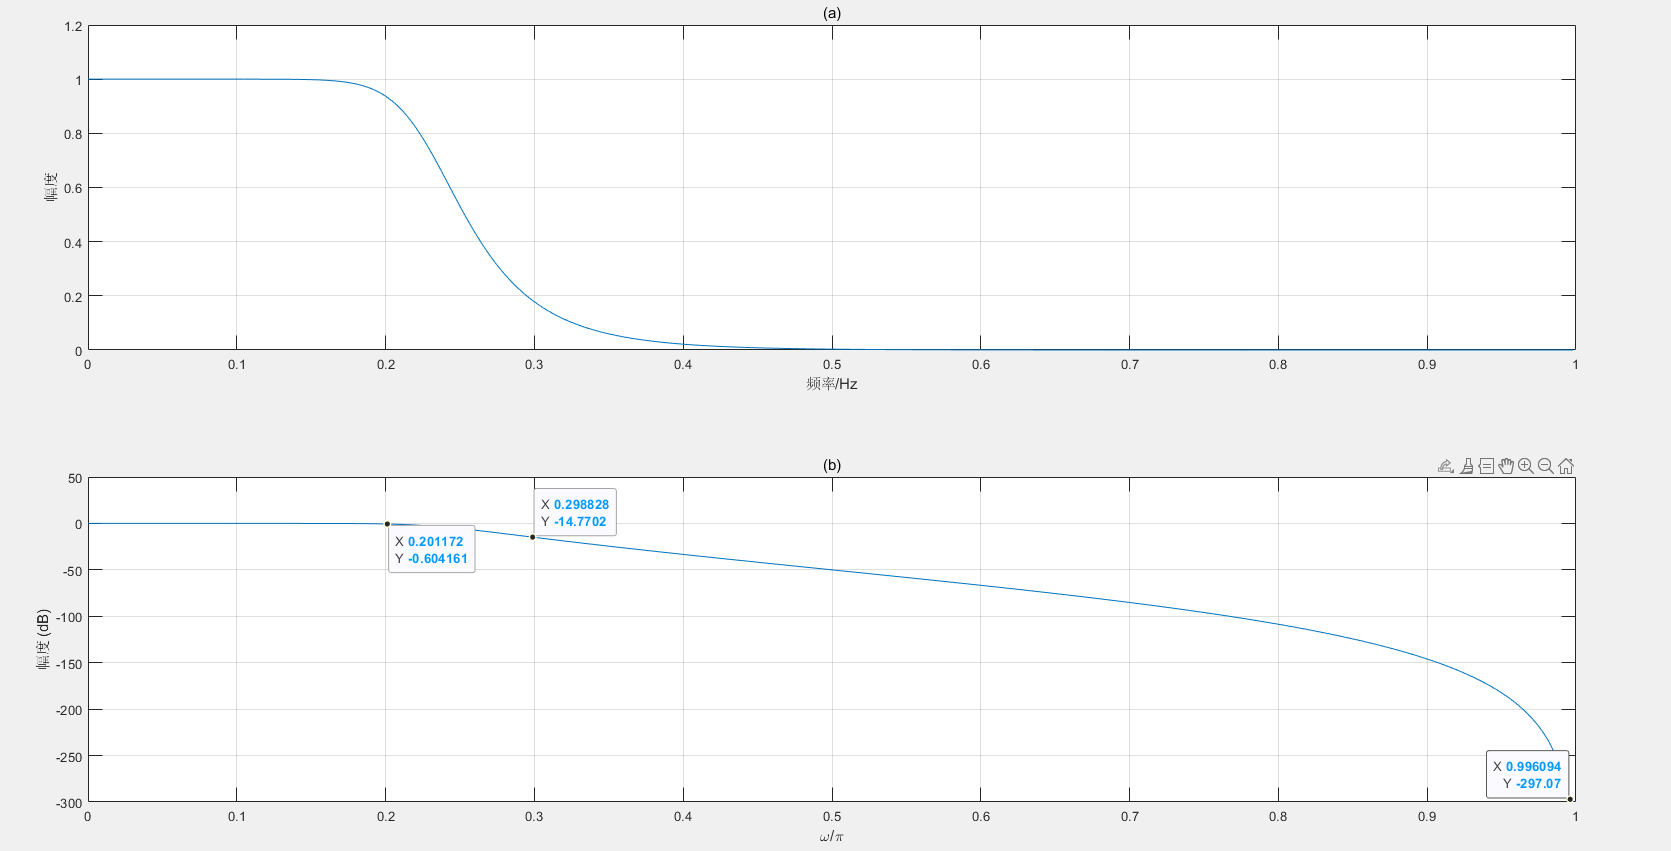
\includegraphics[width=0.9\textwidth]{figures/301.png} % 调整宽度为文本宽度的 80%
        \caption{matlab绘图} %图片标题
        \label{fig:example} % 图片标签,用于引用
\end{figure}

\begin{table}[H]
\centering
\caption{题目一滤波器系数}
\label{tab:filter_coef}
\begin{tabular}{|c|c|c|c|c|c|c|c|}
\hline
\textbf{系数类型} & \multicolumn{7}{c|}{\textbf{系数值}} \\
\hline
\textbf{分子系数} & 0.0007 & 0.0044 & 0.0111 & 0.0148 & 0.0111 & 0.0044 & 0.0007 \\
\hline
\textbf{分母系数} & 1.0000 & -3.1836 & 4.6222 & -3.7795 & 1.8136 & -0.4800 & 0.0544 \\
\hline
\end{tabular}
\end{table}

\subsection{题目二}


% 插入MATLAB代码
\begin{lstlisting}[style=matlab, caption={ MATLAB实现代码}]

% 定义数字高通滤波器的设计参数
wp = 0.8*pi;  % 通带截止频率(归一化,单位:弧度/采样点)
ws = 0.5*pi;  % 阻带截止频率(归一化,单位:弧度/采样点)
Rp = 3;       % 通带最大允许纹波(单位:dB)
Rs = 18;      % 阻带最小衰减(单位:dB)
Fs = 1;       % 采样频率,归一化为 1(简化计算)
Ts = 1/Fs;    % 采样周期,根据采样频率计算,Ts = 1/Fs

% 将数字滤波器的频率转换为模拟滤波器的频率
wp1 = 2*Fs*tan(wp/2); % 使用公式 ωp' = 2*Fs*tan(ωp/2) 将通带频率转换为模拟频率
ws1 = 2*Fs*tan(ws/2); % 使用公式 ωs' = 2*Fs*tan(ωs/2) 将阻带频率转换为模拟频率

% 计算巴特沃斯模拟高通滤波器的阶数和归一化截止频率
[N, Wn] = buttord(wp1, ws1, Rp, Rs, 's'); % 's' 表示设计模拟滤波器,求阶数 N 和截止频率 Wn
disp(['滤波器阶数 N = ', num2str(N)]);   % 输出滤波器阶数 N

% 构建巴特沃斯模拟高通滤波器的传递函数系数
[b, a] = butter(N, Wn, 'high', 's'); % 直接生成阶数为 N 的模拟高通滤波器,'high' 指定高通,'s' 表示模拟域

% 生成巴特沃斯滤波器的零点、极点和增益
[Z, P, K] = buttap(N); % 生成阶数为 N 的巴特沃斯滤波器的零点 Z、极点 P 和增益 K(注:此行未直接使用,可能是遗留代码)

% 使用双线性变换将模拟滤波器转换为数字滤波器
[bz, az] = bilinear(b, a, Fs); % 将模拟滤波器系数 (b, a) 转换为数字滤波器系数 (bz, az)

% 计算数字滤波器的频率响应
[H, W] = freqz(bz, az); % H 为复频率响应,W 为归一化频率(弧度/采样点,范围 [0, π])

% 显示数字滤波器的分子和分母系数
disp('分子系数 bz:'); % 输出提示
disp(bz);             % 输出数字滤波器分子多项式系数
disp('分母系数 az:'); % 输出提示
disp(az);             % 输出数字滤波器分母多项式系数

% 绘制频率响应图并在 ω = 0.5π 处添加标记点
subplot(2,1,1); % 创建 2 行 1 列的子图,选择第一个子图
plot(W*Fs/pi, abs(H), 'b-'); % 绘制线性幅度响应,横轴为实际频率(Hz),因为 Fs = 1,W/pi 范围为 [0, 1]
hold on; % 保持当前图形,以便添加标记点
% 找到 ω = 0.5π 对应的频率点
target_freq = 0.5*pi; % 目标归一化频率
[~, idx] = min(abs(W - target_freq)); % 找到 W 中最接近 0.5π 的索引
scatter(target_freq*Fs/pi, abs(H(idx)), 50, 'r', 'filled', 'Marker', 'o'); % 在 ω = 0.5π 处标记点(红色圆点)
text(target_freq*Fs/pi, abs(H(idx)), sprintf(' (%.3f, %.3f)', target_freq*Fs/pi, abs(H(idx))), 'VerticalAlignment', 'bottom', 'HorizontalAlignment', 'right'); % 添加坐标标签
grid on; % 显示网格线
xlabel('频率/Hz'); % 横轴标签
ylabel('幅度'); % 纵轴标签
title('幅频特性'); % 子图标题
hold off; % 释放图形

subplot(2,1,2); % 选择第二个子图
plot(W/pi, 20*log10(abs(H)), 'b-'); % 绘制 dB 幅度响应,横轴为归一化频率 ω/π,范围 [0, 1]
hold on; % 保持当前图形,以便添加标记点
scatter(target_freq/pi, 20*log10(abs(H(idx))), 50, 'r', 'filled', 'Marker', 'o'); % 在 ω = 0.5π 处标记点(红色圆点)
text(target_freq/pi, 20*log10(abs(H(idx))), sprintf(' (%.3f, %.3f)', target_freq/pi, 20*log10(abs(H(idx)))), 'VerticalAlignment', 'bottom', 'HorizontalAlignment', 'right'); % 添加坐标标签
grid on; % 显示网格线
xlabel('\omega/\pi'); % 横轴标签(归一化频率)
ylabel('幅度 (dB)'); % 纵轴标签
title('幅频特性 (dB)'); % 子图标题
hold off; % 释放图形



\end{lstlisting}

\begin{table}[H]
\centering
\caption{题目二滤波器系数}
\label{tab:filter_coef2}
\begin{tabular}{|c|c|c|c|}
\hline
\textbf{系数类型} & \multicolumn{3}{c|}{\textbf{系数值}} \\
\hline
\textbf{滤波器阶数} & \multicolumn{3}{c|}{N = 2} \\
\hline
\textbf{分子系数} & 0.0778 & -0.1556 & 0.0778 \\
\hline
\textbf{分母系数} & 1.0000 & 1.0708 & 0.3821 \\
\hline
\end{tabular}
\end{table}

\begin{figure}[H] % [H] 表示强制当前位置插入
        \centering
        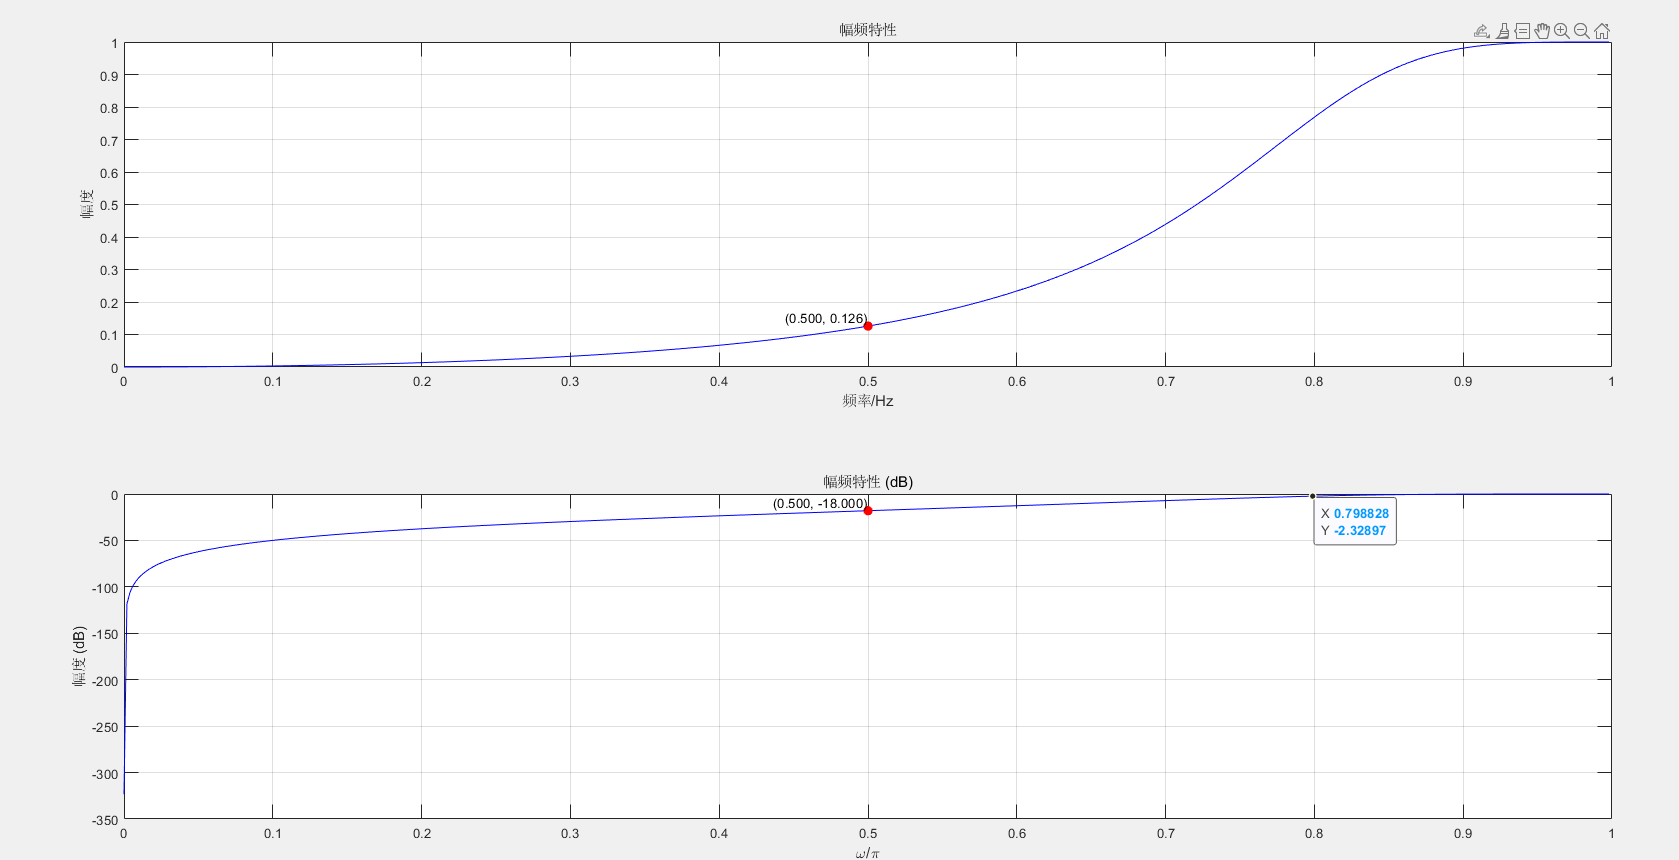
\includegraphics[width=0.9\textwidth]{figures/302.png} % 调整宽度为文本宽度的 80%
        \caption{matlab绘图} %图片标题
        \label{fig:example} % 图片标签,用于引用
\end{figure}

\subsection{题目三}


% 插入MATLAB代码
\begin{lstlisting}[style=matlab, caption={ MATLAB实现代码}]

% 定义数字带通滤波器的设计参数
Fs = 720;       % 采样频率 (Hz)
w1 = 2*Fs*tan(2*pi*60/(2*Fs)); % 计算模拟通带下截止频率 (60 Hz),使用预扭曲公式 w' = 2*Fs*tan(ω/2)
w2 = 2*Fs*tan(2*pi*300/(2*Fs)); % 计算模拟通带上截止频率 (300 Hz),使用预扭曲公式 w' = 2*Fs*tan(ω/2)
w4 = 2*Fs*tan(2*pi*320/(2*Fs)); % 计算模拟阻带上截止频率 (320 Hz),使用预扭曲公式 w' = 2*Fs*tan(ω/2)
w3 = 2*Fs*tan(2*pi*40/(2*Fs));  % 计算模拟阻带下截止频率 (40 Hz),使用预扭曲公式 w' = 2*Fs*tan(ω/2)
wp = [w1 w2];   % 模拟通带频率范围 [w1, w2],用于后续滤波器设计
ws = [w3 w4];   % 模拟阻带频率范围 [w3, w4],用于后续滤波器设计
Rp = 3;         % 通带最大允许纹波 (dB)
Rs = 10;        % 阻带最小衰减 (dB)

% 把模拟滤波器的参数转换为数字滤波器参数
[N, Wn] = buttord(wp, ws, Rp, Rs, 's'); % 计算巴特沃斯模拟带通滤波器的阶数 N 和归一化截止频率 Wn,'s' 表示模拟域
disp(N);        % 输出滤波器阶数 N

% 构建巴特沃斯模拟带通滤波器
[b, a] = butter(N, Wn, 's'); % 生成阶数为 N 的模拟带通滤波器,'s' 表示模拟域

% 使用双线性变换将模拟滤波器转换为数字滤波器
[bz, az] = bilinear(b, a, Fs); % 将模拟滤波器系数 (b, a) 转换为数字滤波器系数 (bz, az),Fs 为采样频率

% 计算数字滤波器的频率响应
[H, W] = freqz(bz, az); % 计算数字滤波器的频率响应,H 为复频率响应,W 为归一化频率 (弧度/采样点)

% 显示数字滤波器的分子和分母系数
disp(bz);       % 输出数字滤波器分子多项式系数
disp(az);       % 输出数字滤波器分母多项式系数

% 绘制频率响应图
subplot(2,1,1); % 创建 2 行 1 列的子图,选择第一个子图
plot(W*Fs/(2*pi), abs(H)); % 绘制线性幅度响应,横轴为实际频率 (Hz),W*Fs/(2*pi) 将归一化频率转换为 Hz
grid on;        % 显示网格线
xlabel('频率/Hz'); % 横轴标签
ylabel('幅度'); % 纵轴标签

subplot(2,1,2); % 选择第二个子图
plot(W*Fs/(2*pi), 20*log10(abs(H))); % 绘制 dB 幅度响应,横轴为实际频率 (Hz)
grid on;        % 显示网格线
xlabel('频率/Hz'); % 横轴标签
ylabel('幅度 (dB)'); % 纵轴标签

\end{lstlisting}

\begin{table}[H]
\centering
\caption{题目三滤波器系数}
\label{tab:filter_coef3}
\begin{tabular}{|c|c|c|c|c|c|c|c|}
\hline
\textbf{系数类型} & \multicolumn{7}{c|}{\textbf{系数值}} \\
\hline
\textbf{分子系数} & 0.3642 & 0.0000 & -1.0926 & -0.0000 & 1.0926 & 0.0000 & -0.3642 \\
\hline
\textbf{分母系数} & 1.0000 & -0.0000 & -1.1162 & 0.0000 & 0.6676 & -0.0000 & -0.1299 \\
\hline
\end{tabular}
\end{table}

\begin{figure}[H] % [H] 表示强制当前位置插入
        \centering
        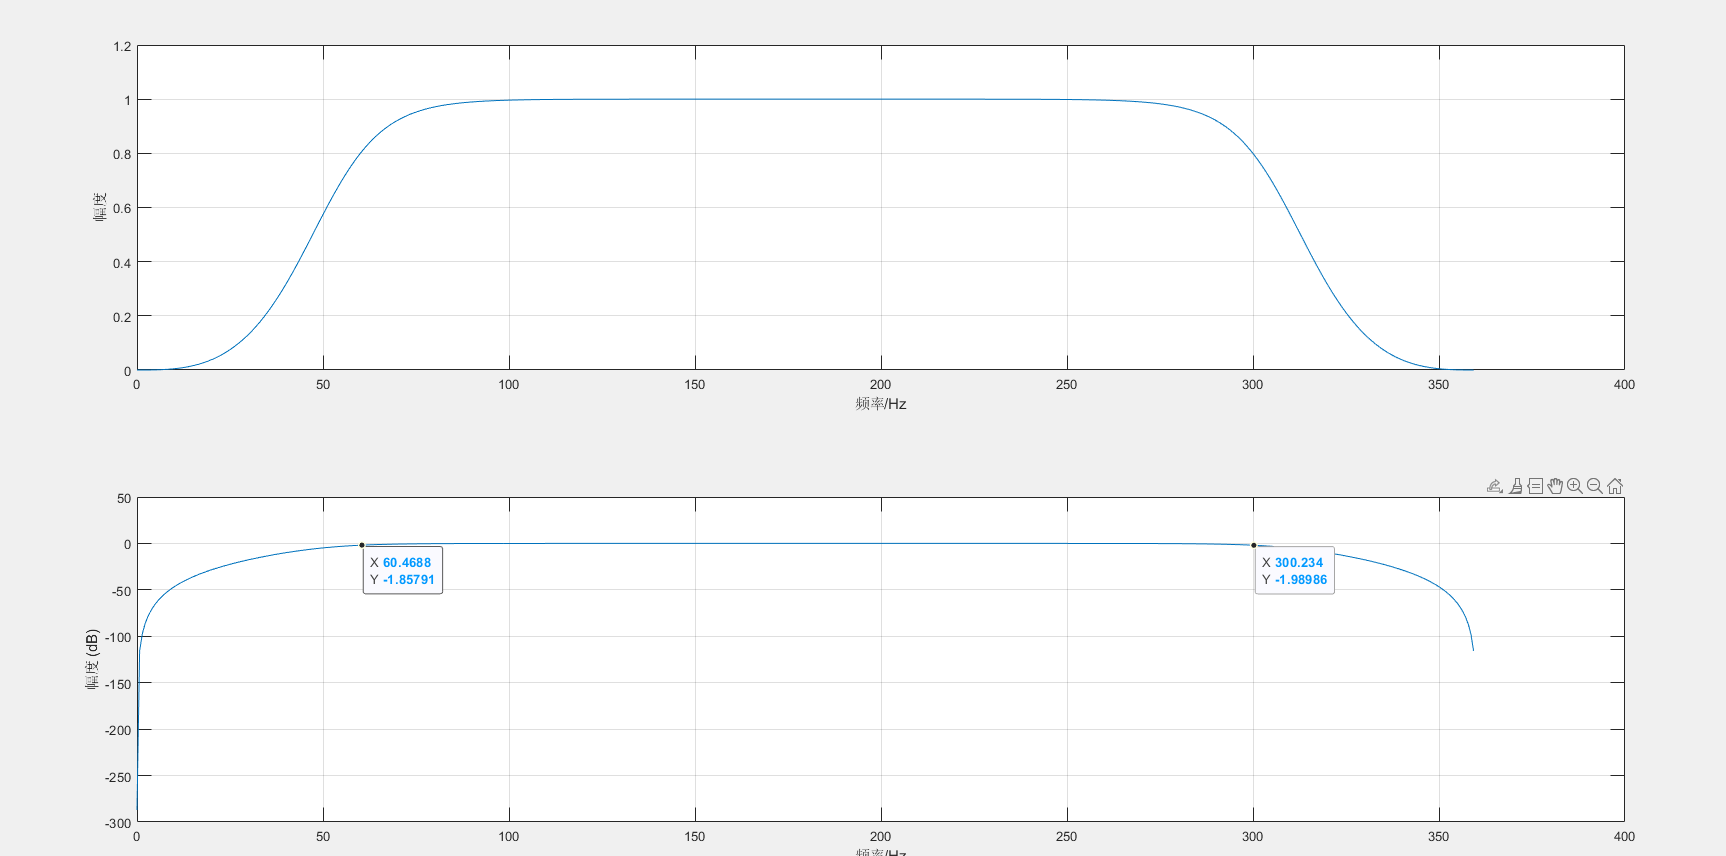
\includegraphics[width=0.9\textwidth]{figures/303.png} % 调整宽度为文本宽度的 80%
        \caption{matlab绘图} %图片标题
        \label{fig:example} % 图片标签,用于引用
\end{figure}



\section{实验小结}

本次实验系统地学习并实践了双线性变换法设计IIR数字滤波器的全过程,主要包括低通、高通和带通巴特沃斯滤波器的设计与分析。通过MATLAB编程实现,掌握了从设计指标出发,经过预扭曲、模拟滤波器设计、双线性变换到数字滤波器实现的完整流程。实验结果表明,所设计的滤波器均能较好地满足幅频特性要求,且通过表格清晰展示了各滤波器的分子、分母系数,便于后续实现和分析。

本实验的主要收获如下:

\begin{itemize}
    \item 熟悉了双线性变换的基本原理及其在数字滤波器设计中的应用,理解了频率预扭曲的重要性。
    \item 掌握了MATLAB中巴特沃斯滤波器的阶数计算、系数求解及频率响应绘制方法。
    \item 通过对比不同类型和参数的滤波器,直观体会了参数变化对滤波器性能的影响。
    \item 学会了如何规范地整理和展示滤波器系数,提升了实验报告的规范性和可读性。
\end{itemize}

本次实验不仅加深了对数字信号处理理论的理解,也提升了实际工程实现能力,为后续更复杂的信号处理任务打下了坚实基础。

\end{document}